\subsection{Einleitung}
\label{sec:fachkonzept-usecase-einleitung}

Um einen Überblick über die Funktionen zu bekommen, die das Planspiel abdecken sollen, wurde das folgende Use-Case-Diagramm erstellt. In diesem Diagramm gibt es zwei Akteure, der Spielleiter und der Spieler. Die einzelnen Funktionen der beiden Akteure werden in den beiden folgenden Kapiteln näher erläutert.

\begin{figure}[h]
  \centering
    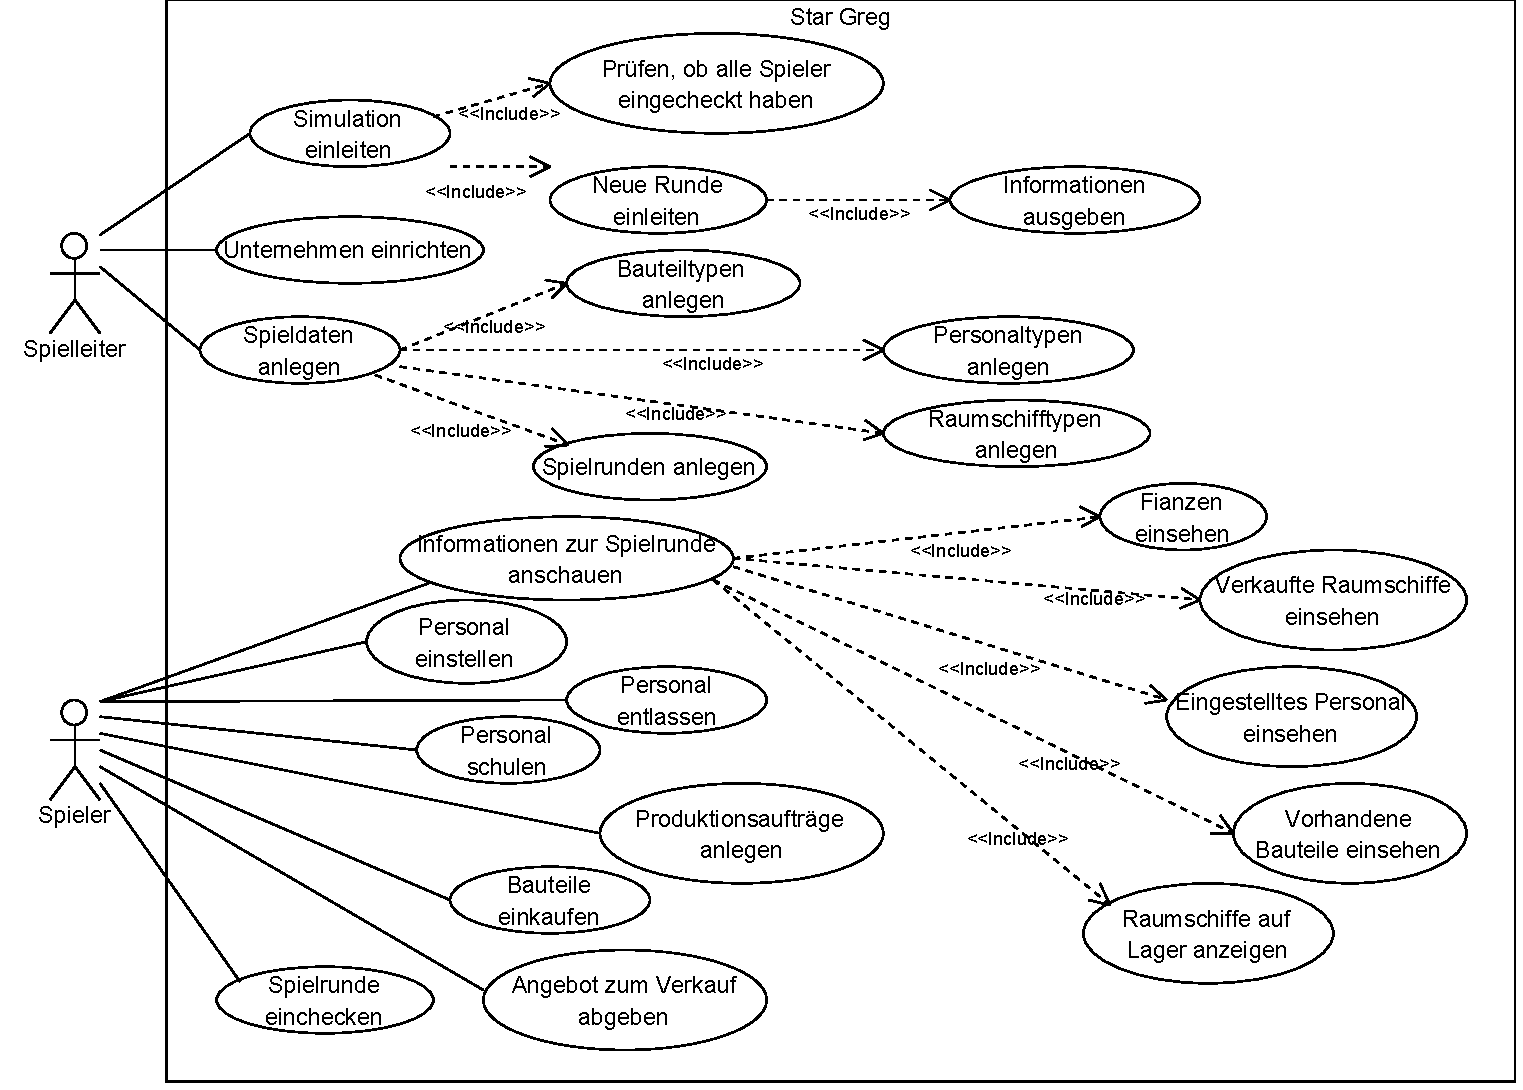
\includegraphics[width=\textwidth]{30_Fachkonzept/10_UseCase/10_Einleitung/diagramm}
  \caption{Use-Case Gesamtdiagramm}
  \label{img:fachkonzept-usecase-einleitung-diagramm}
\end{figure}